\chapter{Технические методы}
\begin{important}
Не стоит забывать, что следующие методы необходимо использовать, по возможности, совместно друг с другом и с методами, перечисленными в предыдущей главе.
\end{important}
\section{Прокси}

\section{VPN}

\section{SSH-туннели}

\section{Настойка браузера}
\begin{important}
Браузер передает огромное количество информации. По отдельности эта информация не представляет никакого интереса, но собранная вместе она может позволить практически со 100\% вероятностью установить вашу личность.
\end{important}
\subsection{Настройка браузера Firefox}
\subsubsection{Предпочитаемые языки}
В меню <<Настройки>> \textrightarrow <<Содержимое>> \textrightarrow <<Языки>> удалите из списка все языки, кроме английского. Несмотря на то, что многие сайты будут теперь использовать по умолчанию английский язык, это повысит вашу анонимность, так ваш браузер станет менее уникальным.
\subsection{Дополнения}
\subsubsection{HTTPS Everywhere}
HTTPS Everywhere --- дополнение для браузеров Firefox и Chrome/Chromium, переадресующее на HTTPS версию сайта, если она доступна. Это позволяет защититься от перехвата передаваемых данных, но не позволяет скрыть сам факт посещения вебсайта. Скачать дополнение можно тут \url{https://eff.org/https-everywhere}.
\subsubsection{BetterPrivacy}
BetterPrivacy --- дополнение для браузера Firefox, позволяющее удалять флеш-куки (Local Shared Objects). Это небольшие куски данных, которые Adobe Flash может сохранять на компьютерах. Ссылка: \url{https://addons.mozilla.org/firefox/addon/betterprivacy/}.
\subsubsection{Ghostery}
Ghostery --- дополнение для браузеров Firefox, Safari, Chrome/Chromium, Opera и Internet Explorer, позволяющее блокировать скрипты, невидимые изображения и прочие методы, используемые многими компаниями для слежки за пользователями. Работает и с LSO, может заменить BetterPrivacy. Сайт: \url{https://www.ghostery.com}.
\subsubsection{TrackerBlock}
TrackerBlock --- дополнение, аналогичное по функционалу Ghostery, доступное для браузеров Firefox, Chrome/Chromium и Internet Explorer. Сайт: \url{http://privacychoice.org/trackerblock}.
\subsubsection{Beef Taco}
Beef Taco --- дополнение для браузера Firefox, позволяющее блокировать куки ресурсов, шпионящих за пользователями. Сайт: \url{http://jmhobbs.github.com/beef-taco/}.
\subsubsection{User Agent Switcher}
User Agent Switcher --- дополнение для браузера Firefox, позволяющее менять заголовок User-Agent, передаваемый браузером. Сайт: \url{http://chrispederick.com/work/user-agent-switcher/}. Вы можете скачать дополнительный список User-Agent здесь \url{http://techpatterns.com/forums/about304.html} и импортировать его в дополнение.
\subsubsection{Smart Referer}
Smart Referer --- дополнение для браузера Firefox, которое позволяет отправлять адрес предыдущей страницы только если она находится на этом же домене. Скачать: \url{https://addons.mozilla.org/firefox/addon/smart-referer/}.
\subsubsection{TrackMeNot}
TrackMeNot --- дополнение для браузеров Firefox и Chrome/Chromium, делающее переодические поисковые запросы к популярным поисковым системам с целью обезличить логи. Сами запросы являются случайными словами из заданной RSS-ленты. Сайт: \url{https://cs.nyu.edu/trackmenot/}.

\section{Анонимные оверлейные сети}
\begin{important}
Никогда не используйте анонимные сети с настройками, которые позволяют использовать Интернет в одном браузере в обход самой сети. В этом случае будет достаточно вставить любое изображение из внешнего Интернета, чтобы получить ваш реальный IP-адрес.
\end{important}
\textbf{Оверлейные сети} --- это такие сети, которые работают поверх другой уже работающей сети.
\subsection{Tor}
\begin{wrapfigure}[9]{r}{0.25\linewidth}

\includegraphics[width=\linewidth]{Tor}
\caption{Логотип Tor}
\end{wrapfigure}
\textbf{Tor} --- анонимная оверлейная сеть, использующая принцип луковой маршрутизации, исходные коды которой распространяются на условиях лицензии BSD\cite{tor_license}.\\
\textbf{Луковая маршрутизация} --- технология анонимного обмена информацией, использующая многократное шифрование и пересылку через цепочки узлов. Каждый луковый маршрутизатор в цепочке удаляет слой шифрования и пересылает сообщение дальше, согласно полученным инструкциям, где все повторится. И так до тех пор, пока сообщение не достигнет адресата. Такое название технология получила из-за сходства данного процесса с очисткой луковицы.\\
\subsubsection{Установка}
Для установки посетите \url{https://torproject.org} или установите пакет с помощью пакетного менеджера вашего дистрибутива.
\subsubsection{Использование}
\subsubsection{Недостатки}
\begin{important}
Не забывайте, что при использовании обычного Интернета через Tor, последняя нода в цепочке (exit-нода) видит трафик нешифрованным.
\end{important}
\begin{enumerate}
\item Медленная скорость работы.
\item Число нод ограничено (не через каждого пользователя Tor проходит трафик), из-за этого IP-адреса exit-нод блокируются на некоторых ресурсах, а в странах с жесткой интернет-цензурой, например, в Китае, блокируются адреса всех нод. Для обхода этой блокировки существуют бриджи --- \url{https://bridges.torproject.org}.
\item Адреса скрытых сервисов сложно запомнить.
\end{enumerate}
\subsection{I2P}
\begin{wrapfigure}[6]{r}{0.25\linewidth}

\includegraphics[width=\linewidth]{I2P}
\caption{Логотип I2P}
\end{wrapfigure}
\textbf{I2P} --- анонимная оверлейная сеть, использующая принцип чесночной маршрутизации, исходные коды которой распространяются на условиях нескольких свободных лицензий\cite{i2p_license}. В отличии от Tor, который в первую очередь направлен на доступ к сайтам обычного интернета (хотя в нем и существуют скрытые сервисы, аналогичные ипсайтам в I2P, а в I2P можно получить доступ к внешнему Интернету, используя аутпрокси), основной целью I2P является доступ именно к скрытым ресурсам --- ипсайтам. Ипсайт от обычного вебсайта отличает только его нахождение в сети I2P.\\
\textbf{Чесночная маршрутизация} --- вариант луковой, отличающийся тем, что несколько <<луковиц>> пересылаются совместно, что усложняет установку авторства сообщений.
\subsubsection{Установка}
Для установки посетите \url{http://i2p2.de} или установите пакет с помощью пакетного менеджера вашего дистрибутива.
\subsubsection{Использование}
После установки настройте свой браузер на использование HTTP-прокси 127.0.0.1:4444 и посетите страницу \url{http://127.0.0.1:7657}. Перед вами консоль маршрутизатора I2P --- место, из которого можно управлять всеми настройками I2P.\\
Для начала перейдите в меню <<Настройки I2P>> (\url{http://127.0.0.1:7657/config} и установите ограничения скорости в соответствии со скоростью вашего интернета. Затем добавьте следующие подписки susidns (\url{http://127.0.0.1:7657/susidns/subscriptions}).
\scriptsize\begin{quote}\begin{verbatim}
http://www.i2p2.i2p/hosts.txt
http://i2host.i2p/cgi-bin/i2hostetag
http://stats.i2p/cgi-bin/newhosts.txt
http://tino.i2p/hosts.txt
http://dream.i2p/hosts.txt
http://biw5iauxm7cjkakqygod3tq4w6ic4zzz5mtd4c7xdvvz54fyhnwa.b32.i2p/uncensored_hosts.txt
http://trevorreznik.i2p/hosts.txt
http://cipherspace.i2p/addressbook.txt
http://hosts.i2p/hosts.cgi?filter=all
http://bl.i2p/hosts2.txt
http://rus.i2p/hosts.txt
http://inr.i2p/export/alive-hosts.txt
http://joajgazyztfssty4w2on5oaqksz6tqoxbduy553y34mf4byv6gpq.b32.i2p/export/alive-hosts.txt
http://qckbnfmbwiueuq2p234wiklgzs6zoc5bbuuubvkr3gb7ziwlsjoa.b32.i2p/list.txt
http://3i2rcjcis3fmy2ylj356qko2eaj5dx5pxlsqc6wqyeirod5uzwzq.b32.i2p/hosts.txt
\end{verbatim}\end{quote}\normalsize
Нажмите <<сохранить>> и <<перезагрузить>>. В I2P отсутствуют корневые DNS-сервера, копия адресной книги хранится на каждом роутере. Данные подписки позволят вам обновлять информацию об адресах ресурсов в своей адресной книге.\\
Остальные настройки можно оставить по умолчанию. Подождите некоторое время для полноценной интеграции с сетью. После интеграции вы сможете полноценно пользоваться сетью. Попробуйте, например, посетить такие ресурсы, как \url{http://forum.i2p} (главный форум, есть рускоязычный раздел), \url{http://rus.i2p} (русская I2P-вики), \url{http://pastethis.i2p} (pastebin-подобный ресурс). Роутер желательно не выключать, так как при его перезапуске потребуется повторная интеграция с сетью.
\subsubsection{Недостатки}
\begin{important}
Не используйте аутпрокси для передачи конфиденциальных данных, владелец аутпрокси видит трафик нешифрованным.
\end{important}
\begin{enumerate}
\item Низкая скорость доступа.
\item Для синхронизации с сетью нужно время.
\end{enumerate}
\subsection{Freenet}
\begin{wrapfigure}[9]{r}{0.25\linewidth}

\includegraphics[width=\linewidth]{Freenet}
\caption{Логотип Freenet}
\end{wrapfigure}
\textbf{Freenet} --- анонимная оверлейная сеть, использующая принципы P2P и F2F и распространяющаяся на условиях GNU GPL v2\cite{freenet_license}. В отличии от Tor и I2P, позволяющих размещать любые ресурсы внутри сети, Freenet по сути представляет собой хранилище статичных данных.\\
\textbf{P2P (Peer-to-peer)} --- компьютерная сеть, в которой все участники равны и выполняют одновременно роль как клиента, так и сервера.\\
\textbf{F2F (Friend-to-Friend)} --- разновидность P2P-сети, в которой все соединения разрешаются только с доверенными узлами.
\subsubsection{Установка}
Для установки посетите \url{https://freenetproject.org} или установите пакет с помощью пакетного менеджера вашего дистрибутива.
\subsubsection{Использование}
\subsubsection{Недостатки}

\section{Анонимный файлообмен}
\subsection{I2Phex}
\subsection{iMule}
\subsection{Mute}
\subsection{Retroshare}
\subsection{Robert}
\subsection{I2PSnark}

\section{Анонимные платежи}
\subsection{Анонимные пластиковые карточки}
\textbf{Анонимные пластиковые карточки} --- карточки, которые зарегистрированны на какого-то другого человека. Обычно являются предоплаченными и их пополнение не возможно. Продаются на различных интернет-форумах и интернет-аукционах.
\subsection{Bitcoin}
\begin{wrapfigure}[6]{r}{0.25\linewidth}

\includegraphics[width=\linewidth]{Bitcoin}
\caption{Логотип Bitcoin}
\end{wrapfigure}
\textbf{Bitcoin} --- открытая электронная анонимная P2P криптовалюта с ограниченной эмиссией. В отличии от прочих валют, у Bitcoin отсутствует владелец и эмиссионый центр, эмиссия выполняется каждым участником сети. Данные о всех транзакциях хранятся в блоках, помещенных в распределенную базу данных.\\
\textbf{Эмиссия} --- выпуск в обращение денежных средств.\\
Bitcoin в экономическом плане напонимает золото, но в отличии от золота его проще передавать, проще хранить, проще проверить подлинность и легко дробить на более мелкие суммы.
\subsubsection{Установка}
Для установки посетите \url{http://bitcoin.org} или установите пакет с помощью пакетного менеджера вашего дистрибутива.
\subsubsection{Использование}
\begin{figure}[h]
\center{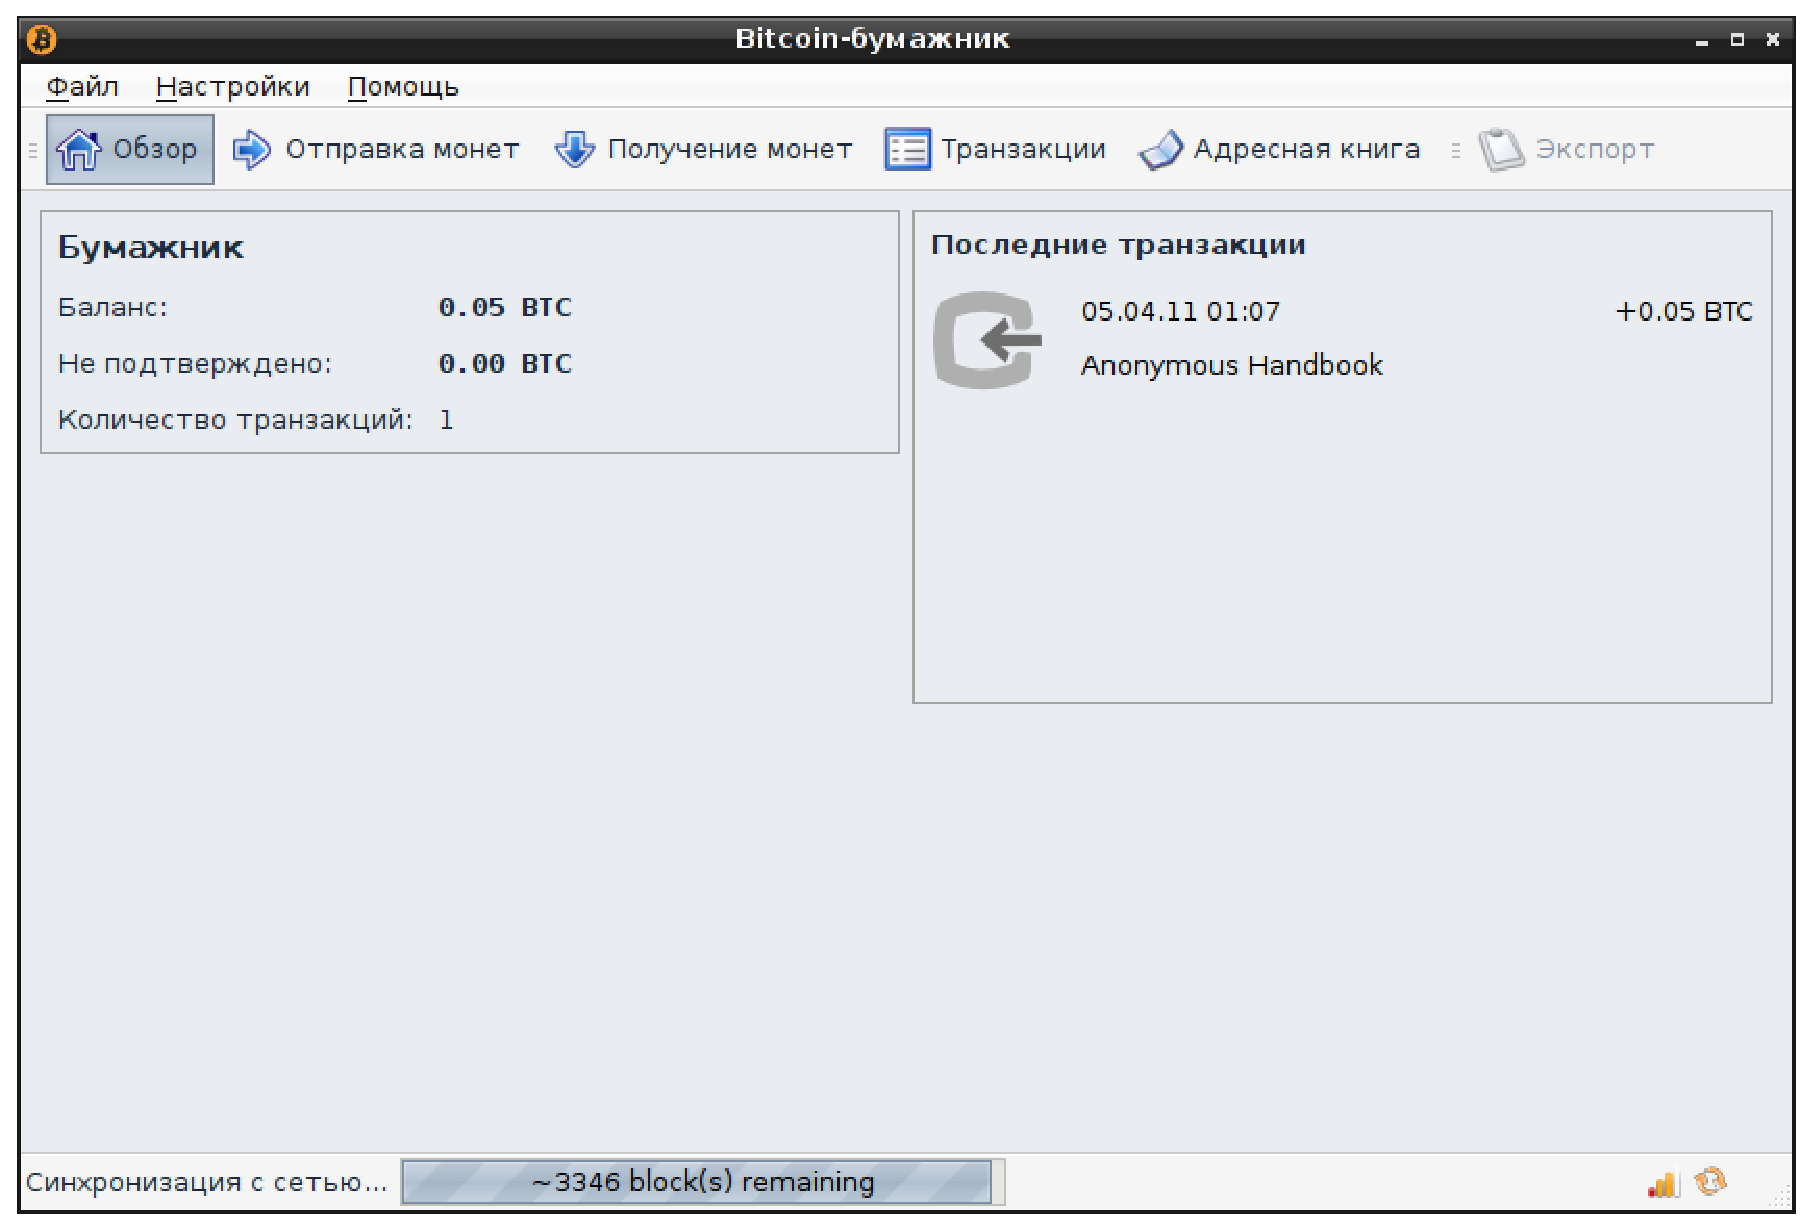
\includegraphics[width=0.75\linewidth]{bitcoin-screen}}
\caption{Интерфейс Bitcoin}
\end{figure}
При первом запуске Bitcoin автоматически создает кошелек. Адрес его можно увидеть на вкладке <<Получение монет>>. Там же вы можете создавать новые адреса, количество их не ограничено.
\subsubsection{Недостатки}
\begin{important}
Кошельки в Bitcoin анонимны, но все транзакции открыты и каждый может их просмотреть через сервисы, подобные \url{http://blockexplorer.com}. Проводите деньги через биржи.
\end{important}
\begin{enumerate}
\item Немгновенные транзакции.
\item Адреса кошельков сложно запомнить.
\item Так как у системы нет владельца, то ни заблокировать кошелек, попавший в руки мошенникам, ни вернуть вам деньги никто не сможет.
\end{enumerate}
\subsection{Прочие платежные системы}

\section{IM-сервисы}
\subsection{I2P-Messenger}
\textbf{I2P-Messenger} --- программа мгновенного обмена сообщениями, работающая в сети I2P. Сайт: \url{http://echelon.i2p/qti2pmessenger}.
\subsection{TorChat}
\textbf{TorChat} --- программа мгновенного обмена сообщениями, работающая поверх Tor. Сайт: \url{https://github.com/prof7bit/TorChat}.
\subsection{JTorChat}
\textbf{JTorChat} --- версия TorChat, переписанная на Java. Сайт: \url{https://github.com/jtorchat/jtorchat}
\subsection{Cryptocat}
\textbf{Cryptocat} --- доступный через браузер чат-сервис с прозрачным шифрованием на Javascript. Сайт: \url{https://crypto.cat}.

\section{Ремейлеры}
\textbf{Ремейлеры} --- сервера, занимающиеся пересылкой сообщений электронной почты по указанному адресу.\\
Ремейлеры бывают псевдонимными (иногда их называют Type 0 или nym) и анонимными. Анонимные делятся на три типа:
\begin{enumerate}
\item Ремейлеры шифропанков
\item Mixmaster 
\item Mixminion
\end{enumerate}
\subsection{Ремейлеры шифропанков}
\textbf{Ремейлеры шифропанков (Type I)} --- ремейлеры, удаляющие из получаемых писем всю информацию, которая может быть использована для идентификации, и пересылающие их на указанный адрес. Зачастую письма можно посылать зашифрованными с помощью GPG. Возможно использование цепочек из нескольких ремейлеров.
\subsection{Mixmaster}
\textbf{Mixmaster (Type II)} --- ремейлеры, требующие установки специальной программы для отправки сообщений. Более безопасны, чем Type I, так как, например, пакеты с сообщениями всегда фиксированного размера, что не позволяет отслеживать письма по размеру. Сайт: \url{http://mixmaster.sourceforge.net}.
\subsection{Mixminion}
\textbf{Mixminion (Type III)} --- ремейлеры, также требующие установки специальной программы, но еще более безопасные, так как используют луковичную маршрутизацию и имеют еще несколько улучшений. Сайт: \url{http://mixminion.net}.

\section{Прием почты}
\subsection{I2P-Mail}
\textbf{I2P-Mail} --- обычный почтовый сервис, находящийся в сети I2P. Позволяет получить почту в домене mail.i2p и i2pmail.org. Пользоваться можно как внутри I2P, так и во внешнем интернете. Адрес: \url{http://hq.postman.i2p}.
\subsection{I2P-Bote}
\textbf{I2P-Bote} --- несовместимая с обычной почтой безсерверная анонимная почта, реализованая в виде плагина для I2P. Сайт: \url{http://i2pbote.i2p}, \url{http://i2pbote.net}.
\subsection{TorMail}
\textbf{TorMail} --- обычный почтовый сервис, работающий как скрытый сервис Tor. Позволяет получить почту в домене tormail.org. Ранее был доступен tormail.net, но он был зарегистрирован через русского регистратора RU-CENTER (nic.ru), который требовал предъявления документов, удостоверяющих личность\cite{tormail}. Адрес: \url{http://jhiwjjlqpyawmpjx.onion}.
\subsection{Privacybox}
\textbf{Privacybox} --- сервис анонимных контактых форм, работающий в I2P, Tor и обычном интернете. Адреса: \url{https://privacybox.de}, \url{http://privacybox.i2p}, \url{http://c4wcxidkfhvmzhw6.onion}.
\subsection{TorPM}
\textbf{TorPM} --- сервис обмена сообщениями, работающий через веб-сайт. Позволяет обмениваться простыми текстовыми сообщениями, напоминающими обычную электронную почту. Адрес: \url{http://4eiruntyxxbgfv7o.onion/pm}.
\subsection{Шифрование почты с помощью GPG}

\section{Шифрование данных}
\subsection{Truecrypt}
\subsubsection{Установка}
Для установки посетите \url{http://truecrypt.org} или установите пакет с помощью пакетного менеджера вашего дистрибутива.
\subsubsection{Использование}
\subsubsection{Недостатки}
\subsection{dm-crypt}
\subsubsection{Использование}
\subsubsection{Недостатки}
\subsection{eCryptfs}
\subsubsection{Использование}
\subsubsection{Недостатки}
\subsection{GPG}
\subsubsection{Установка}
Для установки посетите \url{http://gnupg.org} или установите пакет с помощью пакетного менеджера вашего дистрибутива.
\subsubsection{Использование}
\subsubsection{Недостатки}

\section{Шифрование в IM}
\subsection{Off-the-Record Messaging (OTR)}
\begin{important}
OTR не подходит для шифрования офлайн-собщений, так как подтвержденный вам ключ используется только для передачи других ключей, генерируемых каждую сессию. Ключи, используемые для шифрования сообщений, удаляются после завершения сессии. Сделано это было для того, чтобы нельзя было доказать авторство сообщений после завершения диалога.
\end{important}
\textbf{OTR} --- криптографический протокол, предоставляющий шифрование в системах мгновенного обмена сообщениями. Встроенную поддержку имеют клиенты Adium, climm, MCabber, CenterIM, Phoenix Viewer, Vacuum IM, Jitsi, BitlBee, Spark, с помощью плагина OTR доступен в Pidgin\cite{otr-pidgin}, Kopete\cite{otr-kopete}, Miranda IM\cite{otr-miranda}, Psi+\cite{otr-psi}, Trillian\cite{otr-trillian}, irssi\cite{otr-irssi}, Gajim\cite{otr-gajim}. Также существует OTR localhost AIM Proxy, позволяющая использовать OTR в любом клиенте, но на данный момент поддерживаются только протоколы AIM/ICQ. Сайт: \url{http://cypherpunks.ca/otr/}, плагины для вашего клиента предоставляются сторонними разработчиками.
\subsection{GPG и Jabber}
\textbf{XEP-0027} --- расширение протокола XMPP (Jabber), позволяющее использовать GPG (OpenPGP) для шифрования сообщений\cite{xep-0027}. Поддерживается клиентами Centericq, Gajim, Kopete, Psi и Miranda IM (с помощью плагина).

\section{Стеганография}
\begin{important}
Использование стеганографии само по себе не делает недоступной передаваемую информацию, зная метод (что случается при использовании общедоступной программы) или подвергнув изображение стеганализу можно прочитать скрытую таким образом информацию. Используйте стеганографию совместно со сторонними или встроенными криптографическими утилитами.
\end{important}
\textbf{Стеганография} --- способ тайной передачи информации путем сохранения в тайне самого факта передачи информации. Чаще всего используется совместно с криптографическими методами.
\subsection{steghide}
\subsubsection{Установка}
Для установки посетите \url{http://steghide.sourceforge.net/} или установите пакет с помощью пакетного менеджера вашего дистрибутива.
\subsubsection{Использование}
\begin{figure}[ht!]
\vspace{-4ex}
\centering
\subfigure[]{
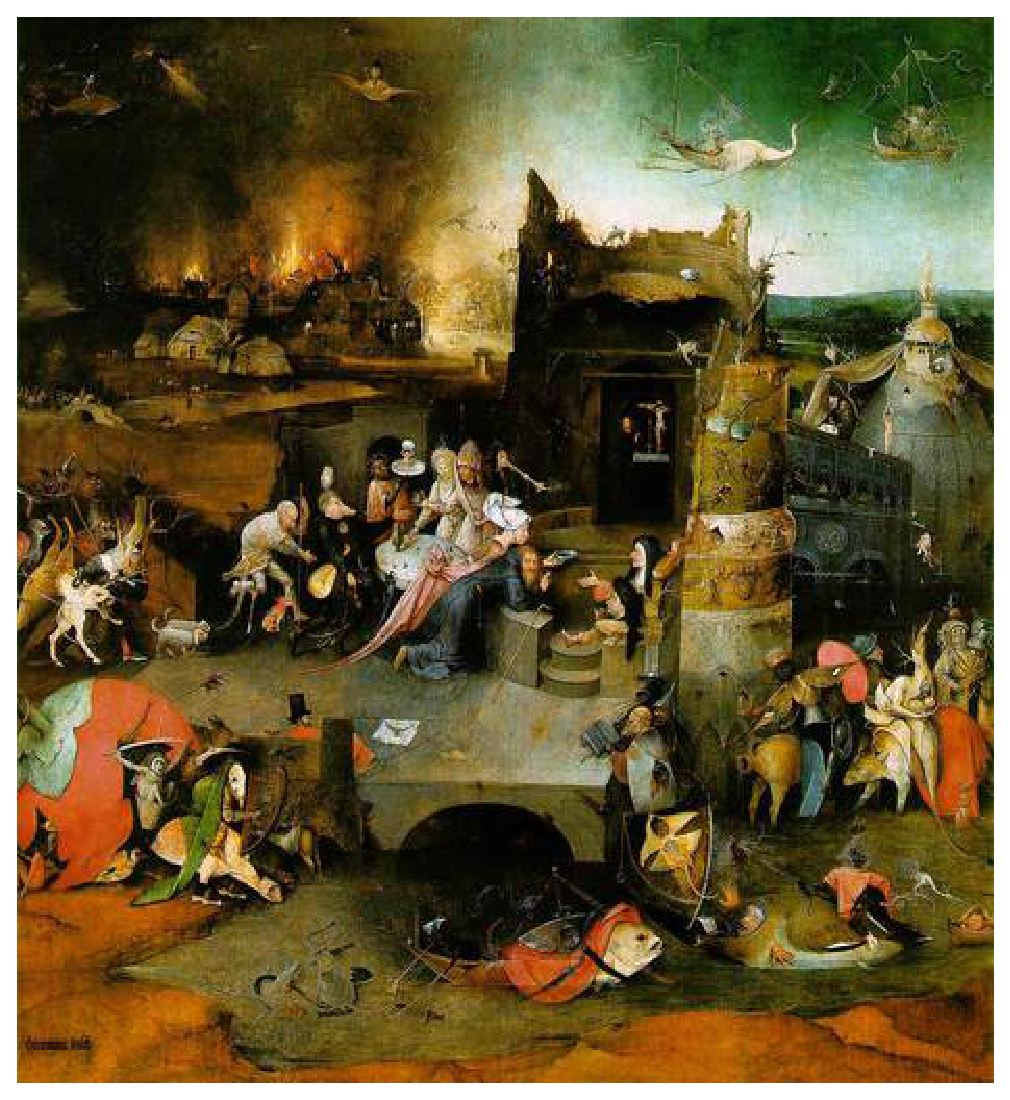
\includegraphics[width=0.25\linewidth]{original}
\label{fig:original}
}
\hspace{4ex}
\subfigure[]{
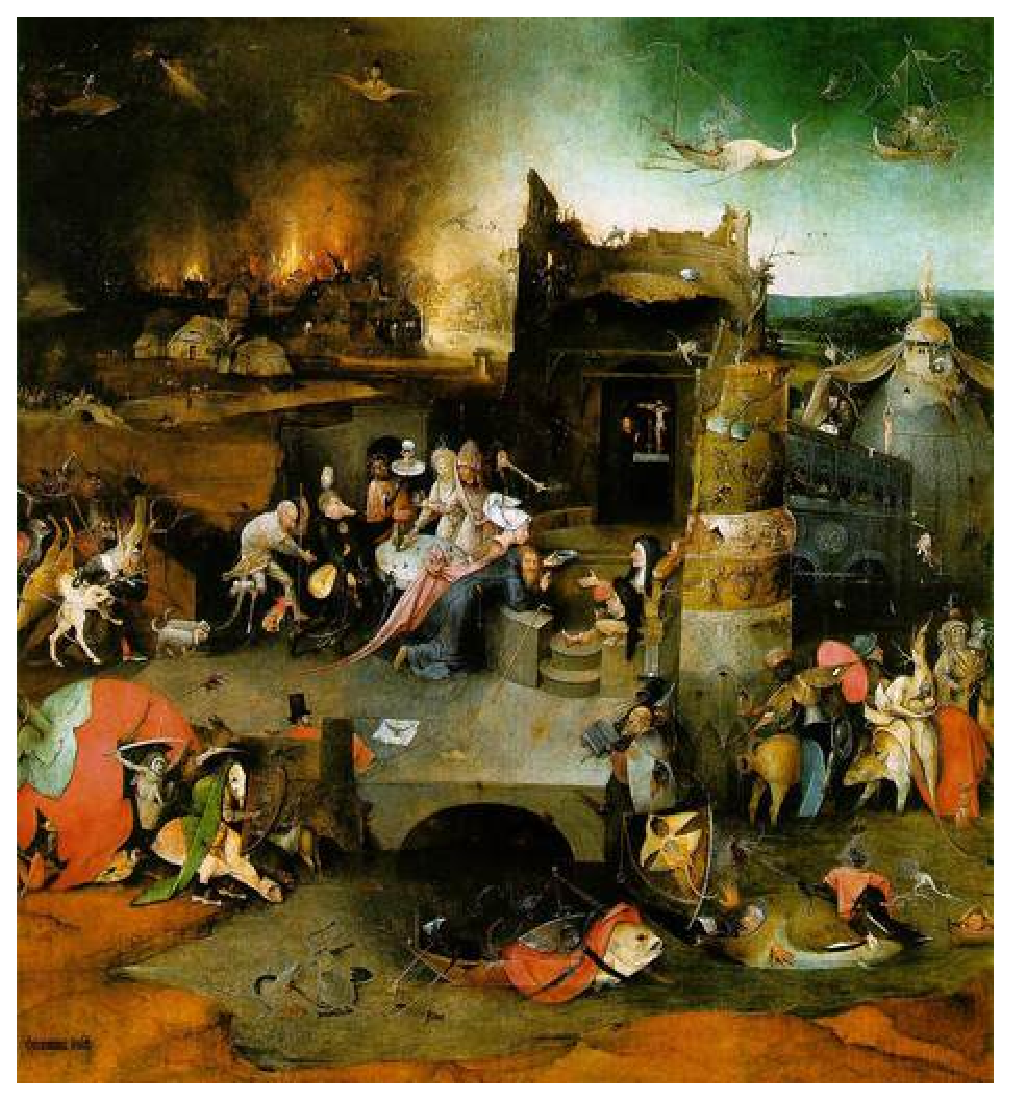
\includegraphics[width=0.25\linewidth]{steghide1}
\label{fig:steghide1}
}
\hspace{4ex}
\subfigure[]{

\includegraphics[width=0.25\linewidth]{steghide2}
\label{fig:steghide2}
}
\caption{Использование steghide: 
\subref{fig:original} исходное изображение; 
\subref{fig:steghide1} в изображении закодирована фраза <<Feci quod potui, faciant meliora potentes>> с паролем <<cogitoergosum>>; 
\subref{fig:steghide2}} разница между изображениями.
\end{figure}
Вставка данных в изображение:
\begin{lstlisting}
steghide embed -cf "coverfile.jpg" -ef "embedfile.txt" -sf "stegofile.jpg" -p "password"
\end{lstlisting}
coverfile.jpg --- файл, в который вставляются данные.\\
embedfile.txt --- файл, который вставляется в изображение.\\
stegofile.jpg --- файл со вставленным изображением.\\
password --- пароль.\\\\
Извлечение данных:
\begin{lstlisting}
steghide extract -sf "stegofile.jpg" -p "password" -xf "extractfile.txt"
\end{lstlisting}
stegofile.jpg --- файл со вставленным изображением.\\
password --- пароль.\\
extractfile.txt --- файл, в который нужно записать извлеченные данные.
\subsubsection{Недостатки}
\subsection{OpenStego}
\subsubsection{Установка}
Для установки посетите \url{http://openstego.sourceforge.net/} или установите пакет с помощью пакетного менеджера вашего дистрибутива.
\subsubsection{Использование}
\begin{figure}[h]
\center{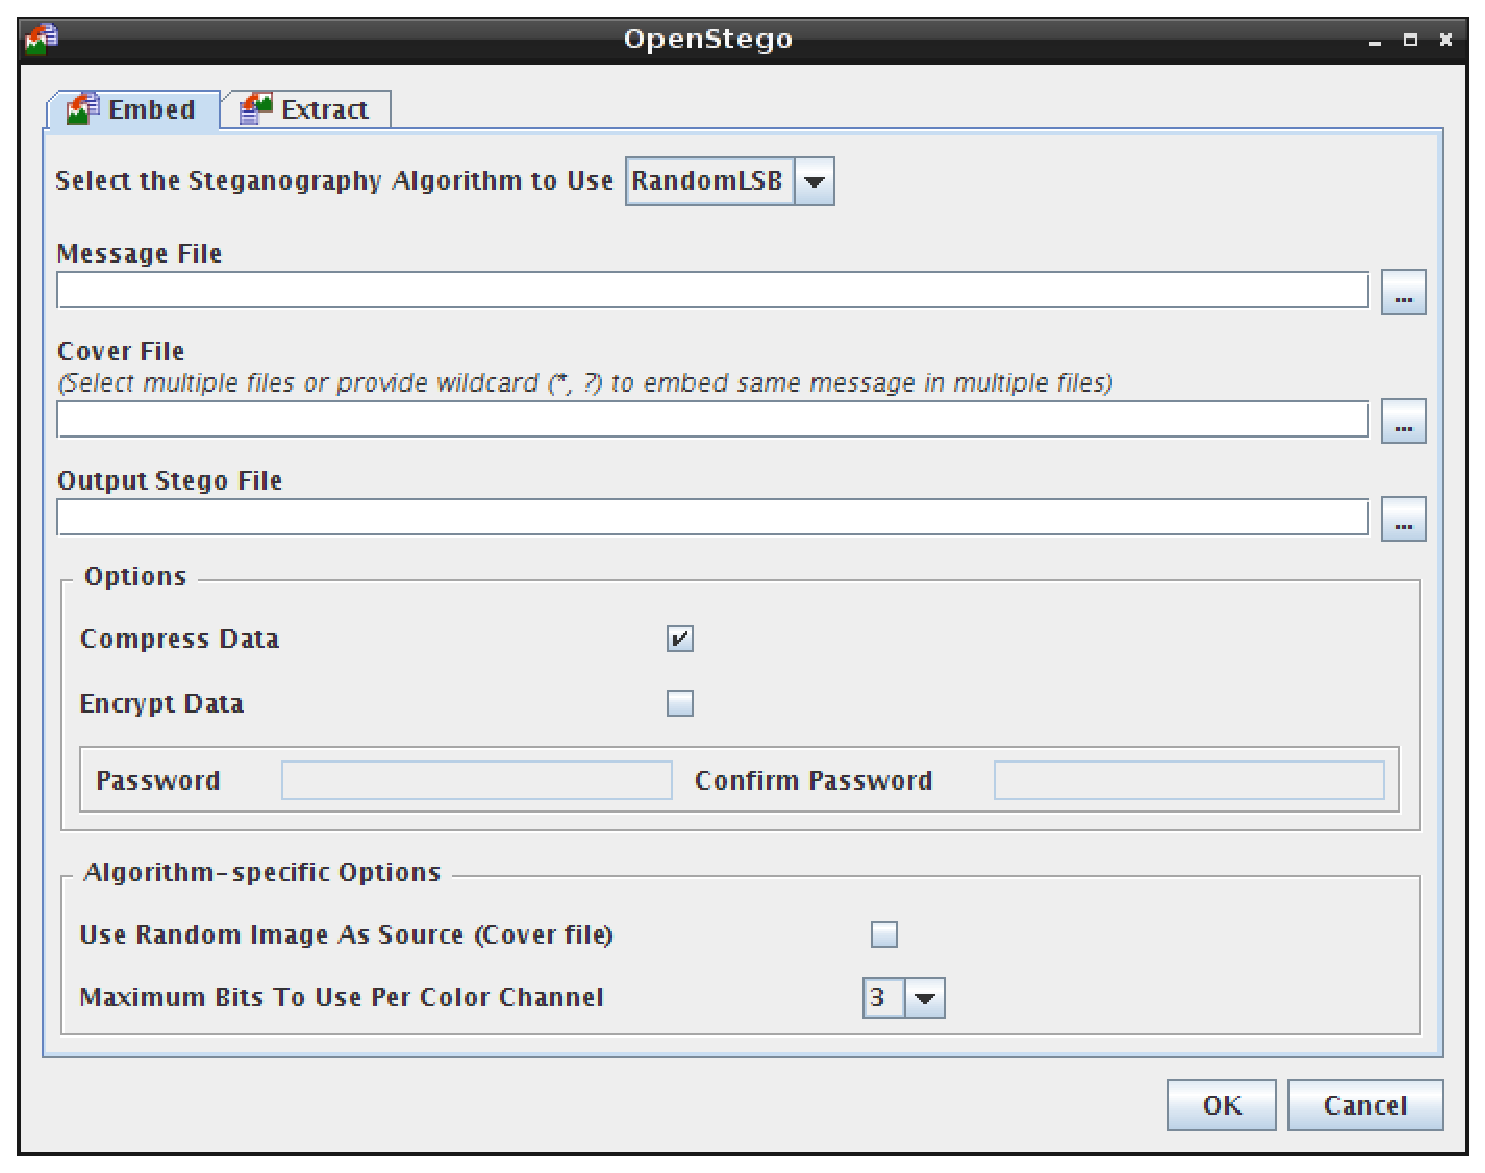
\includegraphics[width=0.75\linewidth]{openstego}}
\caption{Интерфейс OpenStego}
\end{figure}
\begin{figure}[ht!]
\vspace{-4ex}
\centering
\subfigure[]{
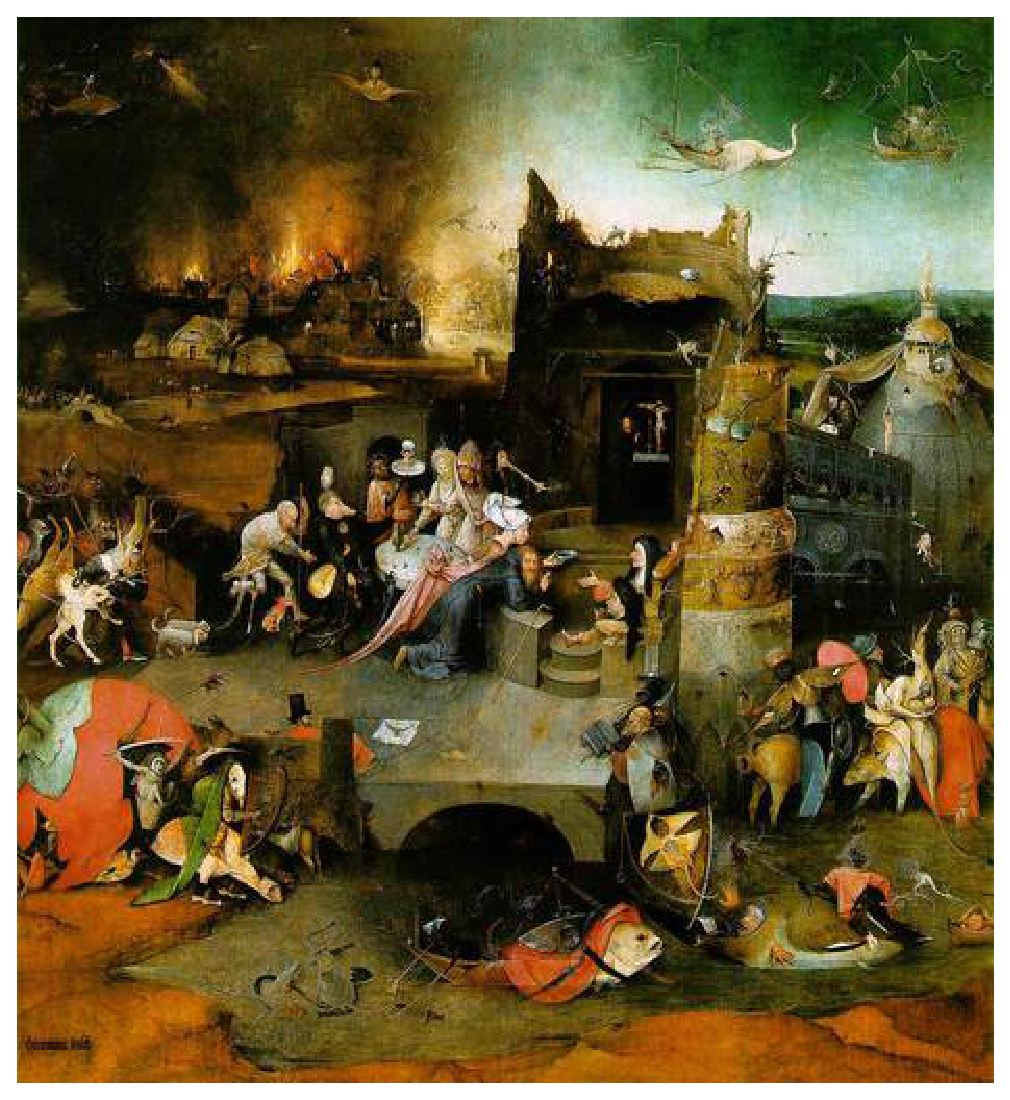
\includegraphics[width=0.25\linewidth]{original}
\label{fig:original}
}
\hspace{4ex}
\subfigure[]{
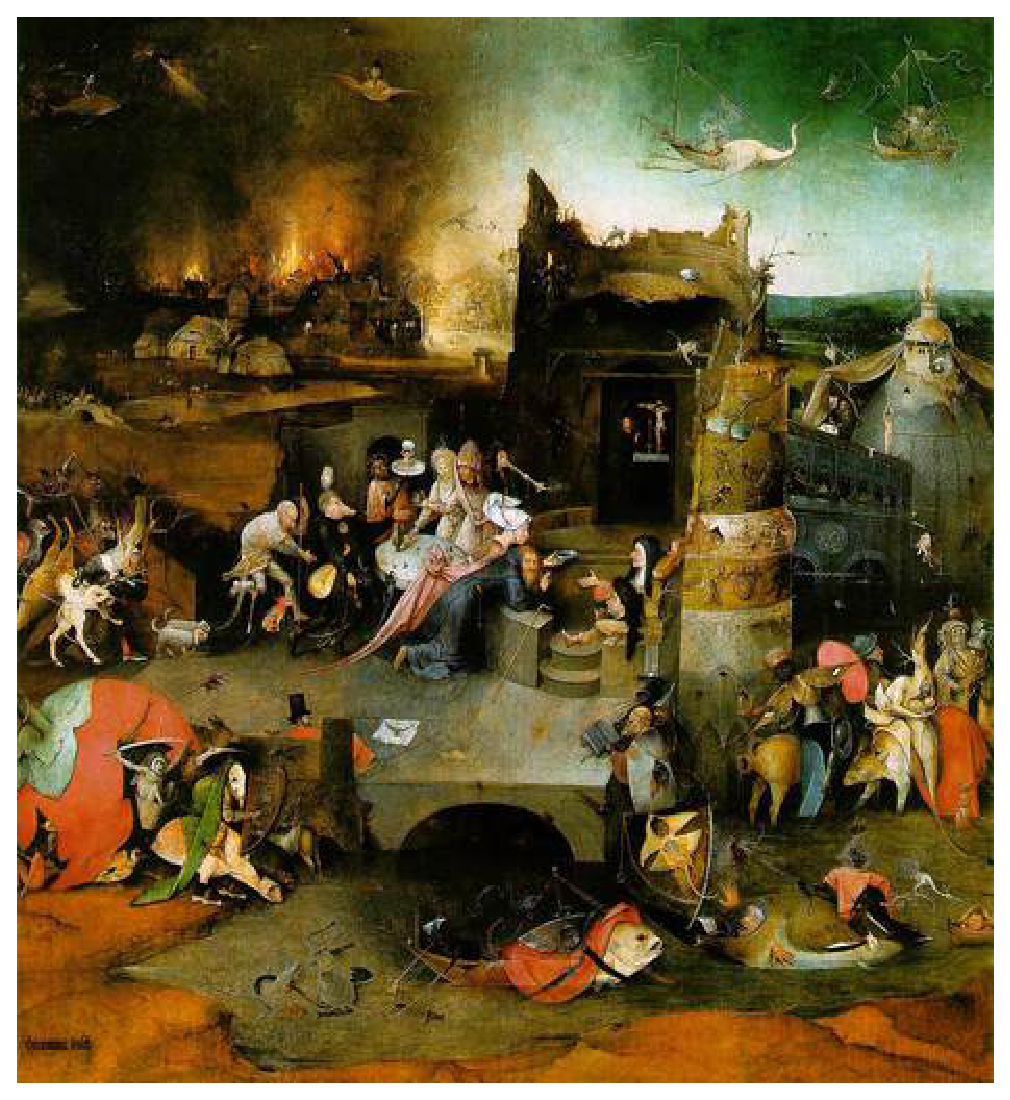
\includegraphics[width=0.25\linewidth]{openstego1}
\label{fig:openstego1}
}
\hspace{4ex}
\subfigure[]{

\includegraphics[width=0.25\linewidth]{openstego2}
\label{fig:openstego2}
}
\caption{Использование OpenStego:
\subref{fig:original} исходное изображение;
\subref{fig:openstego1} в изображении закодирована фраза <<Feci quod potui, faciant meliora potentes>> без пароля;
\subref{fig:openstego2}} разница между изображениями.
\end{figure}
\subsubsection{Недостатки}
\subsection{StegoShare}
StegoShare специально приспособлен для того, чтобы прятать несколько файлов в нескольких изображениях и расшаривать их в P2P-сетях.
\subsubsection{Установка}
Для установки посетите \url{http://stegoshare.sourceforge.net} или установите пакет с помощью пакетного менеджера вашего дистрибутива.
\subsubsection{Использование}
\begin{figure}[h]
\center{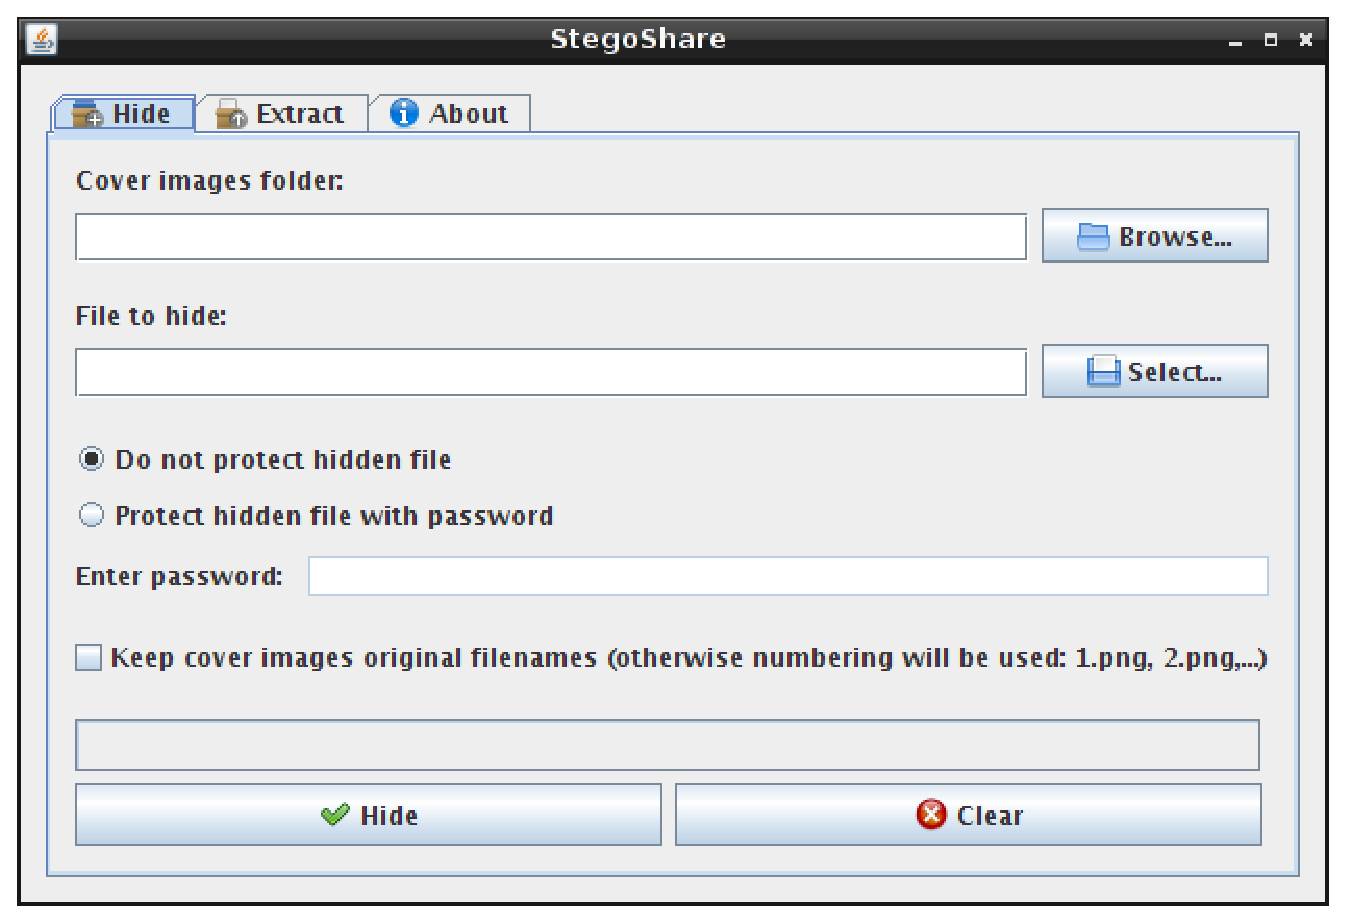
\includegraphics[width=0.75\linewidth]{stegoshare}}
\caption{Интерфейс StegoShare}
\end{figure}
\begin{figure}[ht!]
\vspace{-4ex}
\centering
\subfigure[]{
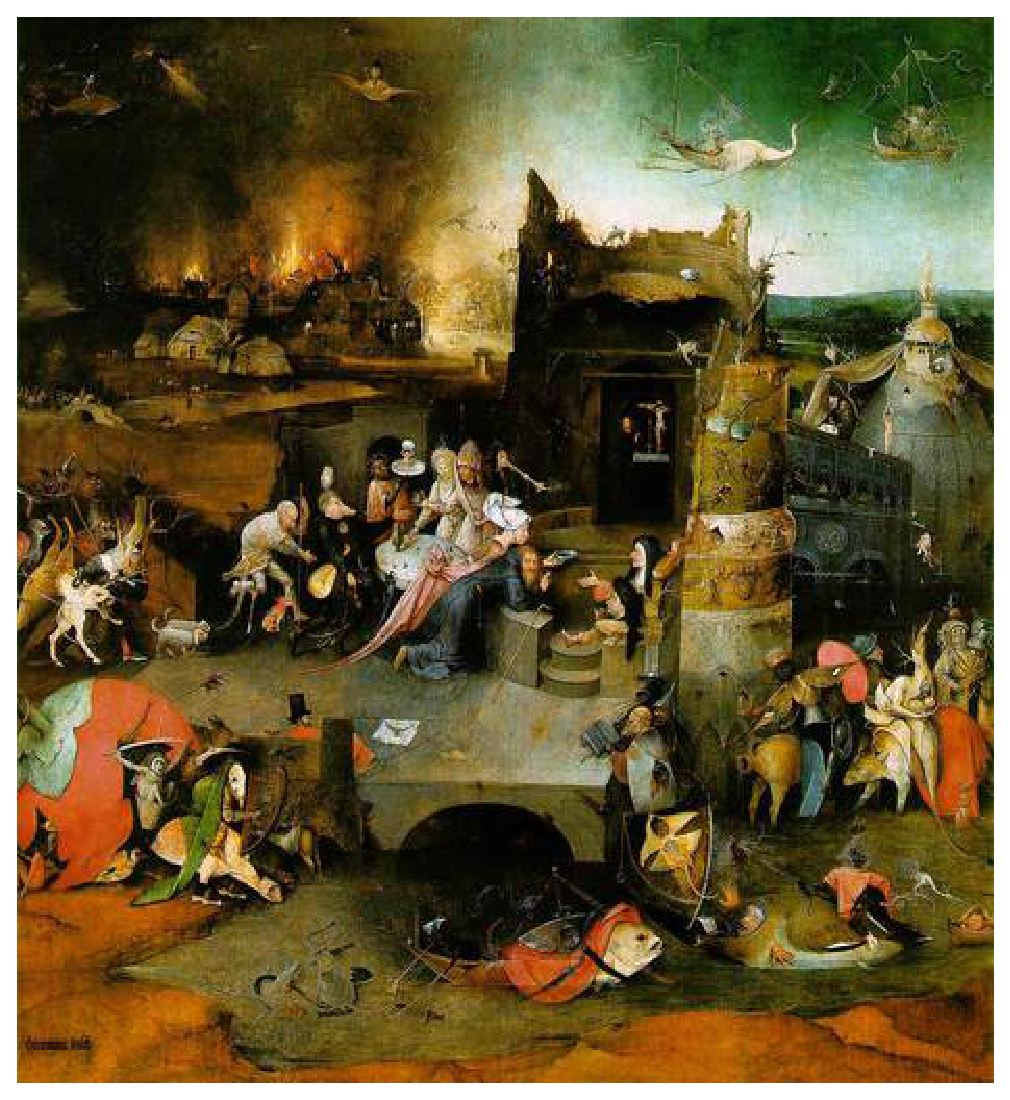
\includegraphics[width=0.25\linewidth]{original}
\label{fig:original}
}
\hspace{4ex}
\subfigure[]{
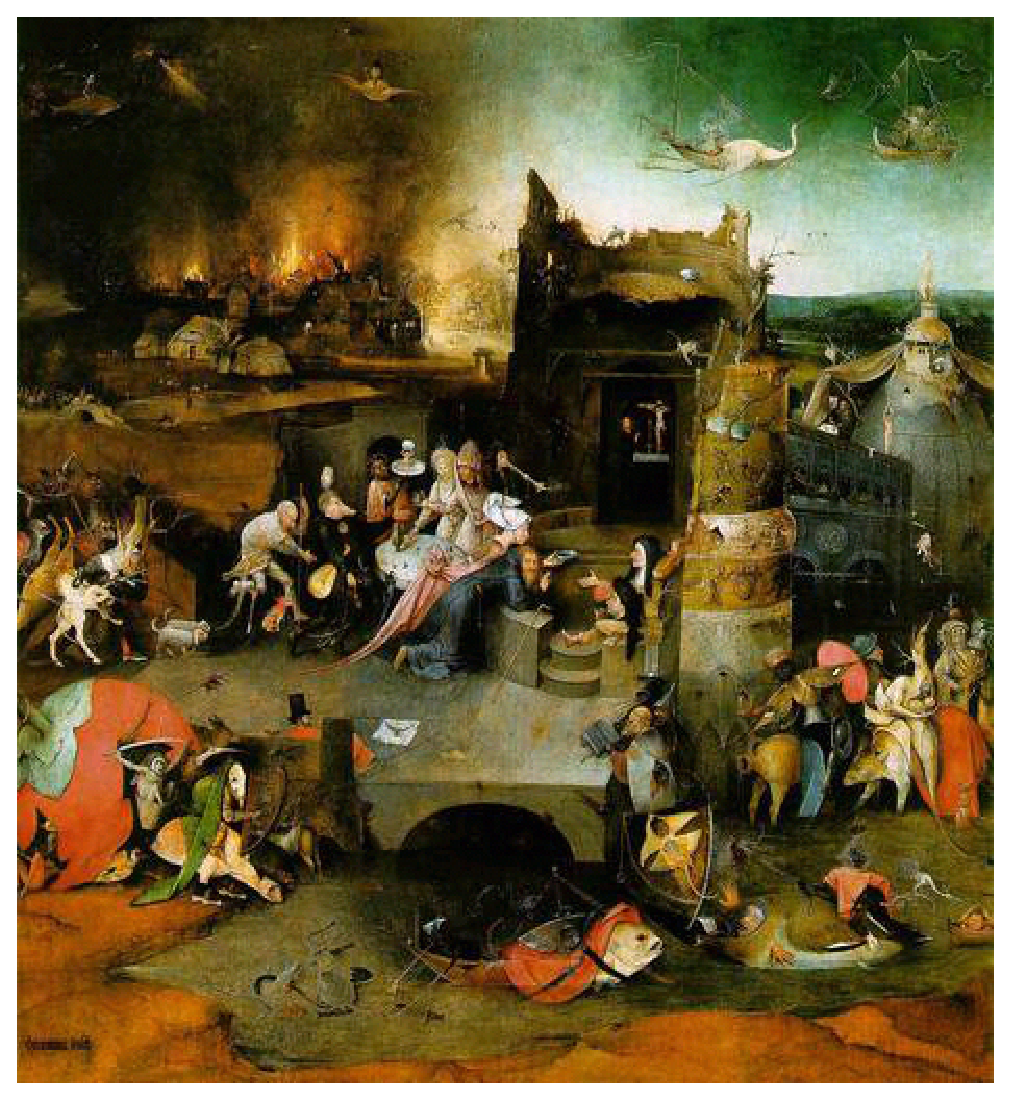
\includegraphics[width=0.25\linewidth]{stegoshare1}
\label{fig:stegoshare1}
}
\hspace{4ex}
\subfigure[]{

\includegraphics[width=0.25\linewidth]{stegoshare2}
\label{fig:stegoshare2}
}
\caption{Использование StegoShare:
\subref{fig:original} исходное изображение;
\subref{fig:stegoshare1} в изображении закодирована фраза <<Feci quod potui, faciant meliora potentes>> без пароля;
\subref{fig:stegoshare2}} разница между изображениями.
\end{figure}
\subsubsection{Недостатки}
\subsection{Желтые точки}
\begin{wrapfigure}[9]{r}{0.25\linewidth}
\includegraphics[width=\linewidth]{dots}
\caption{Желтые точки. Изображение: Parhamr}
\end{wrapfigure}
При печати материалов (например, листовок) не стоит забывать, что многие принтеры кодируют микроточками информацию о времени печати и о серийном номере принтера \cite{eff_dots}. Данная информация может быть использована для установления личности авторов отпечатков. Список принтеров, размещающих и не размещающих желтые точки смотрите в отчете Electronic Frontier Foundation\cite{eff_list}.

\section{Альтернативные DNS}
\subsection{Namecoin}
\textbf{Namecoin} --- распределенная система доменных имен, основанная на Bitcoin, хранящая в блоках информацию о доменах. Она сохранила многие плюсы Bitcoin, например, никто не может заблокировать ни один домен. В настоящее время возможно получение доменов в зоне .bit, однако воспользоваться ими смогут только те, кто предварительно настроил свой компьютер.
\subsubsection{Установка}
\begin{important}
Стоит заменить, что все методы, не подразумевающие установку собственного резолвера, не безопасны. При использовании прокси-серверов владелец может перехватывать все данные, а при использовании открытых DNS-серверов владелец может установить сам факт посещения конкретного сайта.
\end{important}
Существует несколько способов использовать Namecoin.
\begin{enumerate}
\item Использовать открытый прокси, адреса которых перечислены здесь \url{https://dot-bit.org/How_To_Browse_Bit_Domains#List_of_App_proxies}.
\item Использовать альтернативный DNS-сервер с поддержкой Namecoin, адреса открытых серверов перечислены здесь \url{https://dot-bit.org/How_To_Browse_Bit_Domains#List_of_DNS_servers}.
\item Использовать DNS-суффикс \url{https://dot-bit.org/How_To_Browse_Bit_Domains#List_of_DNS_suffixes}.
\item Использовать веб-прокси \url{https://dot-bit.org/How_To_Browse_Bit_Domains#List_of_Web_proxies}.
\item Использовать BIND с NamecoinToBind. Подробнее \url{https://github.com/khalahan/NamecoinToBind}.
\item Использовать ncproxy совместно с Tor (наилучший вариант): \url{https://dot-bit.org/forum/viewtopic.php?p=1448#p1448}.
\item Использовать NmcSocks (тоже возможно использование вместе с Tor): \url{https://github.com/itsnotlupus/nmcsocks}.
\end{enumerate}
\subsubsection{Недостатки}
\subsection{OpenNIC}
\subsection{Собственный кеширующий DNS сервер}

\section{Хранение паролей}
\begin{important}
Не используйте один и тот же пароль на нескольких ресурсах и не используйте простых паролей. Не храните пароли в открытом виде, пользуйтесь менеджерами паролей, которые используют криптографические методы для предотвращения кражи ваших паролей.
\end{important}
\subsection{KeePassX}
\textbf{KeePassX} (не путать с KeePass) --- кроссплатформенный менеджер паролей, распространяющийся на условиях GNU GPL v2, форк KeePass. Сайт: \url{https://keepassx.org}.
\subsection{KeePass}
\textbf{KeePass} --- кроссплатформенный (через Mono) менеджер паролей. Сайт: \url{http://keepass.info}.
\subsection{KWallet}
\textbf{KWallet} --- кроссплатфоменный менеджер паролей, разрабатывающийся в рамках проекта KDE. Сайт: \url{http://utils.kde.org/projects/kwalletmanager/}.
\subsection{Revelation}
\textbf{Revelation} --- менеджер паролей для GNU/Linux и *BSD. Сайт: \url{http://revelation.olasagasti.info}.

\section{Безопасное удаление файлов}
\begin{important}
Простое удаление файлов оставляет возможность для восстановления, так как файлы на самом деле никуда не исчезают, а просто помечаются как удаленные и на этот сектор диска становится возможна запись.
\end{important}
\subsection{shred}
\textbf{shred} --- утилита из пакета GNU coreutils, позволяющая переписывать указанные файлы несколько раз, что делает практически невозможным их восстановление. Сайт GNU coreutils: \url{http://www.gnu.org/software/coreutils}.
\subsubsection{Использование}
\begin{lstlisting}
shred -u "файл"
\end{lstlisting}
\subsubsection{shreg}
shreg --- графический интерфейс для shred. Сайт: \url{https://github.com/arxell/shreg}.
\subsection{wipe}
\textbf{wipe} --- аналогичная утилита для UNIX-подобных систем, работающая по тому же принципу. Сайт: \url{http://lambda-diode.com/software/wipe/}.
\subsubsection{Использование}
\begin{lstlisting}
wipe "файл"
\end{lstlisting}

